\documentclass[10pt,conference,letterpaper]{IEEEtran}
\usepackage{times,amsmath}
\usepackage{cite} 
\usepackage{url}
\usepackage{graphicx}
%
\title{MyGesture: A Laptop Control System over WiFi via Android device using gestures}
%
\author{%
% author names are typeset in 11pt, which is the default size in the author block
{Pranjal Singh{\small $~^{\#1}$}, Vaibhav{\small $~^{\#2}$}, R.K. Ghosh{\small $~^{\#3}$} }%
% add some space between author names and affils
\vspace{1.6mm}\\
\fontsize{10}{10}\selectfont\itshape
% separate superscript on following line from affiliation using narrow space
$^{\#}$\,Dept. of Computer Science \& Engineering, IIT Kanpur\\
Kanpur, India\\
\fontsize{9}{9}\selectfont\ttfamily\upshape
%
% in the following email addresses, separate the superscript from the email address 
% using a narrow space \,
% the reason is that Acrobat Reader has an option to auto-detect urls and email
% addresses, and make them 'hot'.  Without a narrow space, the superscript is included
% in the email address and corrupts it.
% Also, removed ~ from pre-superscript since it does not seem to serve any purpose
$^{1}$\,spranjal@iitk.ac.in\\
$^{2}$\,vaibhavv@iitk.ac.in\\
$^{3}$\,rkg@iitk.ac.in%
% add some space between email and affil
\vspace{1.2mm}\\
\fontsize{10}{10}\selectfont\rmfamily\itshape
% 20080211 CAUSAL PRODUCTIONS
% separated superscript on following line from affiliation using narrow space \,
\fontsize{9}{9}\selectfont\ttfamily\upshape
% removed ~ from pre-superscript since it does not seem to serve any purpose

}

\begin{document}
\maketitle
\thispagestyle{plain}
\pagestyle{plain}

\begin{abstract} 
Smart device based markets are constantly expanding and increasingly becoming popular. For smart modern-day living, interactive mobile applications have become increasingly important especially on interaction of people and modern-day devices. In this work, we have come up with a WiFi based mobile device interactive application in Android that can use gestures and sensors of Android device to control a laptop including keyboard and mouse control. The goal of this work is to explore how to make use of the most of the android gestures and sensors for our most common interactions with a laptop. Using this framework, we demonstrate how easy and useful it becomes to control a laptop using an android device. The android device just acts like a smart remote control of a laptop.\\\\
\end{abstract}
% NOTE keywords are not used for conference papers so do not populate them
\begin{keywords}
android, wifi, laptop, gesture, sensor, keyboard, mouse\\
\end{keywords}

\section{Introduction}
Initially, the mobile phones were developed basically for voice related communication, after which they transformed into sms and data based communication device but now-a-days the scenario has changed altogether, voice communication has now become just one aspect of a mobile device. There are several other aspects related to a mobile device which have become major focus of interest nowadays. Two such major factors are gesture recognition and wireless communication. Both of these functionalities are already implemented in the modern day devices but are only in the hands of manufacturers  and not in the hands of users. This is mainly due to absence of most of the users in app development, the users donot have self control on the apps and have to do with the already developed apps. \\\\
But now, since the release of android-based open source mobile phones in the market and presence of active developers a user can access every feature directly. He can manufacture for himself customized and interactive applications to do almost anything and they can  also program other hardware components like camera, sensors, touchpad, etc.\\\\
Modern day devices such as mobile phones and computer’s have become inevitable parts of ones’ life. One of the important aspect of modern day technology is to remotely monitor these devices. Currently we already have many Remote Control applications which provides an easy control over devices and can monitor these devices easily and quickly.  MyGesture is basically an Android-based Mobile Application for controlling a Target system such as a PC. User can almost have full access of the Target PC. MyGesture surrounds the Client and Server application. The Server application has been implemented in JAVA and Client application in Android. As both JAVA and Android are open source platforms, they allows the development of new ideas and tests them with a set of open standards. One can use MyGesture to remotely control a laptop via mouse, keyboard, interactive gestures, shake, and much more.\\\\
Laptop is a computer with mobility as compared to a desktop computer. Smart phones differ from portable computers which in turn evolved from desktop computers. A smart phone is an advanced mobile phone that offers variety of features such as computing ability and remote connectivity.\\\\ Wi-Fi, also spelled Wifi or WiFi, is a technology that allows an electronic device to exchange data or connect to the internet wirelessly using microwaves in the 2.4 GHz and 5 GHz bands.\\ Android is an operating system based on the Linux kernel and designed primarily for touchscreen mobile devices such as smart-phones and tablet computers. The user interface of Android is based on direct manipulation, using touch inputs that loosely correspond to real-world actions, like swiping, tapping, pinching, and reverse pinching to manipulate on-screen objects. Internal hardware such as accelerometers, gyroscopes, and proximity sensors is used by some applications to respond to additional user actions, for example adjusting the screen from portrait to landscape depending on how the device is oriented.
\begin{figure*}
\centering
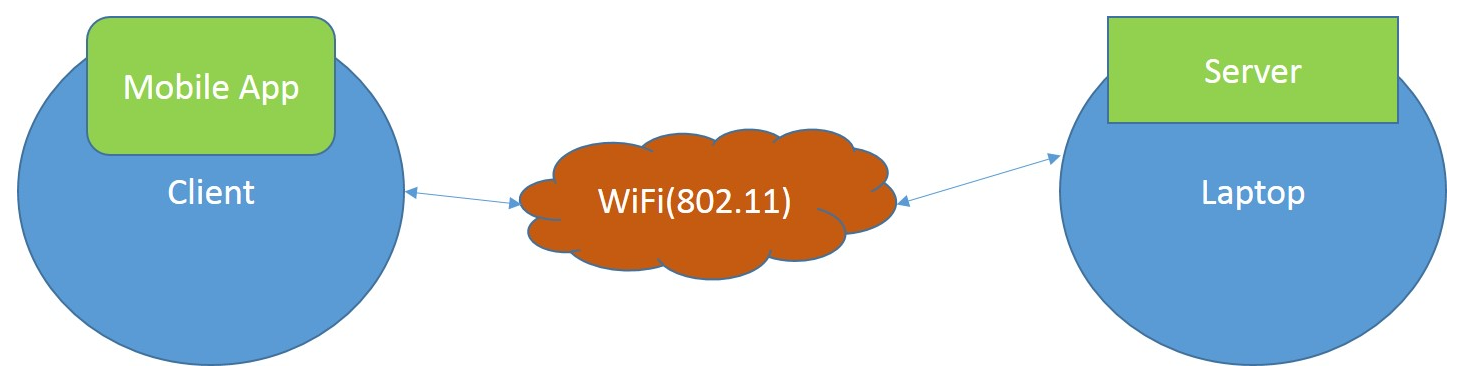
\includegraphics[width=120mm,height=35mm]{1.eps}
\caption{An outline of our framework}
\end{figure*} 

This paper describes MyGesture, an Android application using which a user can connect to any computer having Server Application running on it and can control most of its basic operations.\\\\
The rest of the paper is organized as follows. Section 2 describes some of the previous work, Section 3 describes our implementation and features showing screenshots for easy understanding. Section 4 describes our implementation details. Section 5 describes future work. Section 6 concludes current work and Section 7 is acknowledgement followed by the last section which contains the references.

\section{Related Work}
Wieser (1991) founded the area of pervasive, also called, ubiquitous, computing, where he predicted that one day the computers would be integrated into everyday objects and would develop to a extent that they would interact with people seamlessly. A number of research projects have come up which relate the use of the cell phone as a remote monitor and controller. [1] Describes an architecture for remote controlling based on Android. As per work done by [1], there can be different types of possibilities which exist, to establishing connectivity between the Target PC and the Mobile Client such as USB-Interface, Java Sockets, etc. Each of them has its own consequences. The work done by [2] describes an architecture for remote controlling based on Bluetooth. It has been implemented in J2ME and the target PC is Windows based. It takes the help of two technologies for creating connection: COM ports and JSR-82. By default, the personal Computers do not support the JSR-82 API. Work done by [3] uses the C\#.Net technology for client and server. They have established the connection using 802.11 link. The client is a PDA. A large number of projects and initiatives have been designed that allow remote control between devices. Also there are some initiatives that aim to control mobile devices. But a large number of them lacks in use of open source platforms. So, with this work, we present an initiative that covers this particular area of interest.
The proposed platform is flexible and scalable. This paper focuses on controlling through Android Platforms. This is an open platform that allows using other technologies (also open). In addition, Android platform allow the development of new ideas easily and test them with a set of open standards [4]. The prototype generated as implementation of the proposed architecture will be provided also as free software. According to data released by Nielsen [5], half of the consumers who recently purchased a Smartphone chose an Android Smartphone. 


\section{Features}
The features which we have implemented are summarized in the following table.
\begin{table}[!h]
\centering

    \caption{Features at a glance}     % NOTE!  caption goes _before_ the table contents !!
    \label{tab:font-sizes}

    \begin{small}
    \begin{tabular}{|l|l|l|}
    \hline
    \cline{2-3}
    {\bfseries  Gesture/Input}         & {\bfseries API used}     & {\bfseries Laptop Output}           \\
	\hline
    Keyboard Input	&	Key Press  	& Key Press     \\
    &  Detect&\\
    \hline
    Touch Input 	&	Pad Movement 	& Simulates Mouse     \\
    (Mouse) &  &\\   
    \hline
    Double Finger Scroll	&	Two finger touch	& Normal Scrolling	\\
          
    \hline
    Pinch to zoom	& Two-finger  & Zoom-In and 	\\
                   &  Movement on screen            & Zoom-Out \\
             
    \hline
    Three finger 	&	Three finger 	& Window Switch     \\
    touch &  touch detect&\\
     \hline
    Four finger 	&	Four finger 	& Screen Snapshot    \\
    touch &  touch detect & Capture\\         
    \hline
    Two finger touch at 		&	Two finger touch detect	&	Close current 		\\
    top right and  &   & window\\
    bottom right &  &\\
    \hline
	 Two finger touch at  &	Two finger touch detect	&	Minimize current 		\\
	 bottom left and  &  &\\
	 bottom right &  &window\\
    \hline
     Two finger touch at 	&	Two finger touch detect	&	Maximize current   \\
     top left and  &    & window \\
     top right &  &\\
     \hline
     Two finger touch at 	&	Two finger touch detect	&	Opens Task   \\
     top left and  &    & Manager \\
     bottom right &  &\\
     \hline
     Two finger touch at 	&	Two finger touch detect	&	Locks Windows   \\
     top right and  &    &  Screen \\
     bottom left &  &\\
     \hline
     Volume key press	&	Button Press Detection	&	Changes volume   \\
      &    &  of Media Player \\
     \hline
     Shake Device	&	Accelerometer Sensor	&	Plays next music  \\
      &    &  track \\
     \hline
     Two finger touch at 		&	Two finger touch detect	&	Print Command 		\\
    top left and  &   & \\
    bottom left &  &\\
    \hline
    Hard Press 		&	Pressure Detect	&	Previous slide 		\\
    \hline
    \end{tabular}
    \end{small} 
\end{table}

\begin{figure*}
\centering
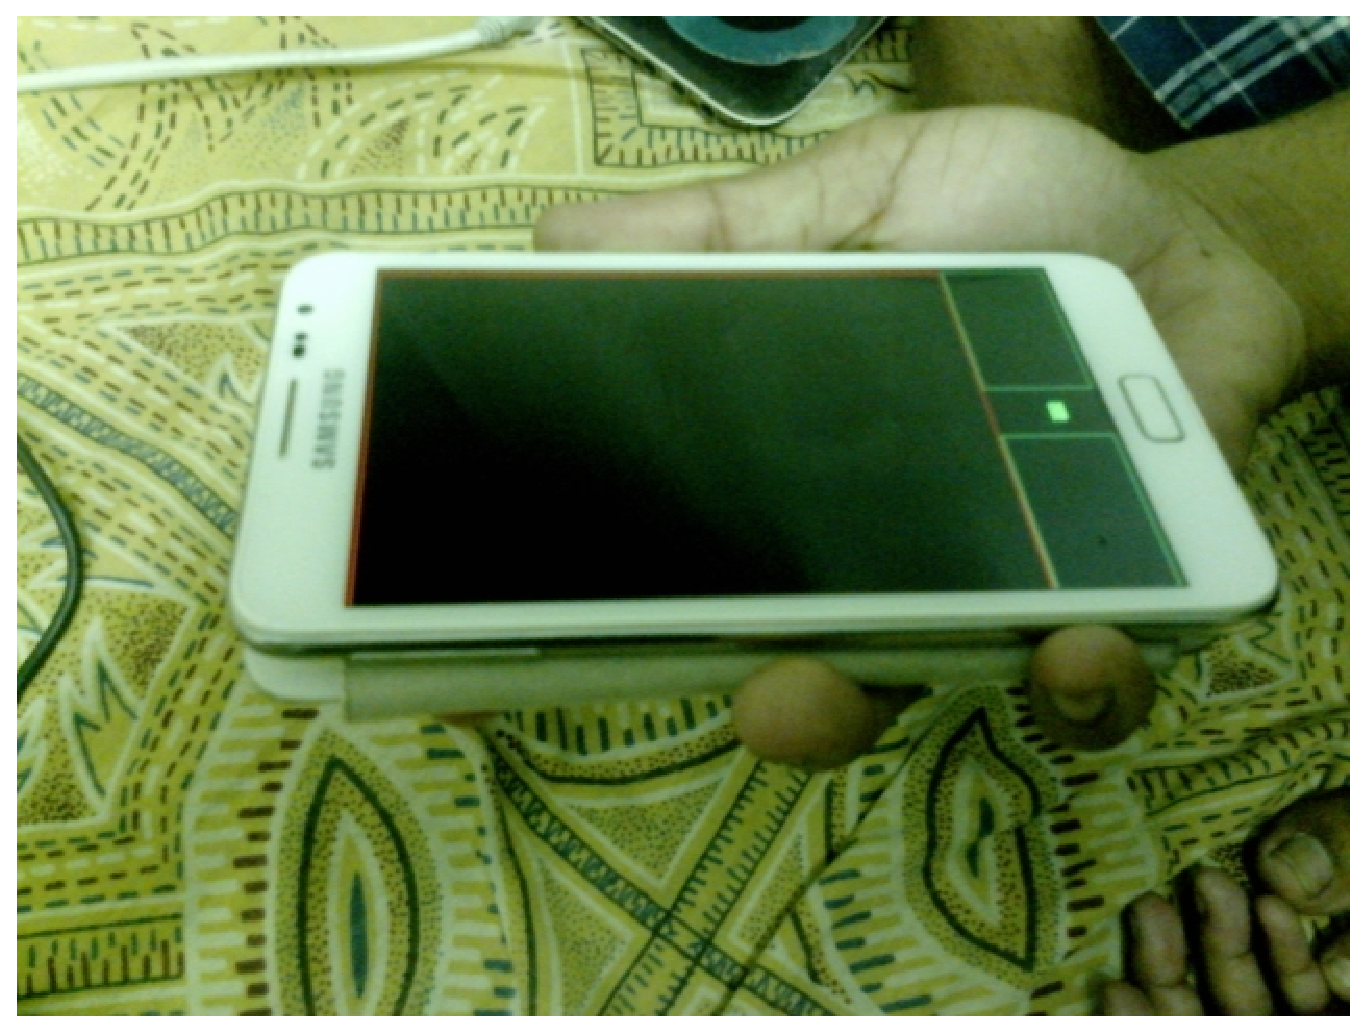
\includegraphics[width=120mm,height=45mm]{2.eps}
\caption{Shake}
\end{figure*}
\begin{figure*}
\centering
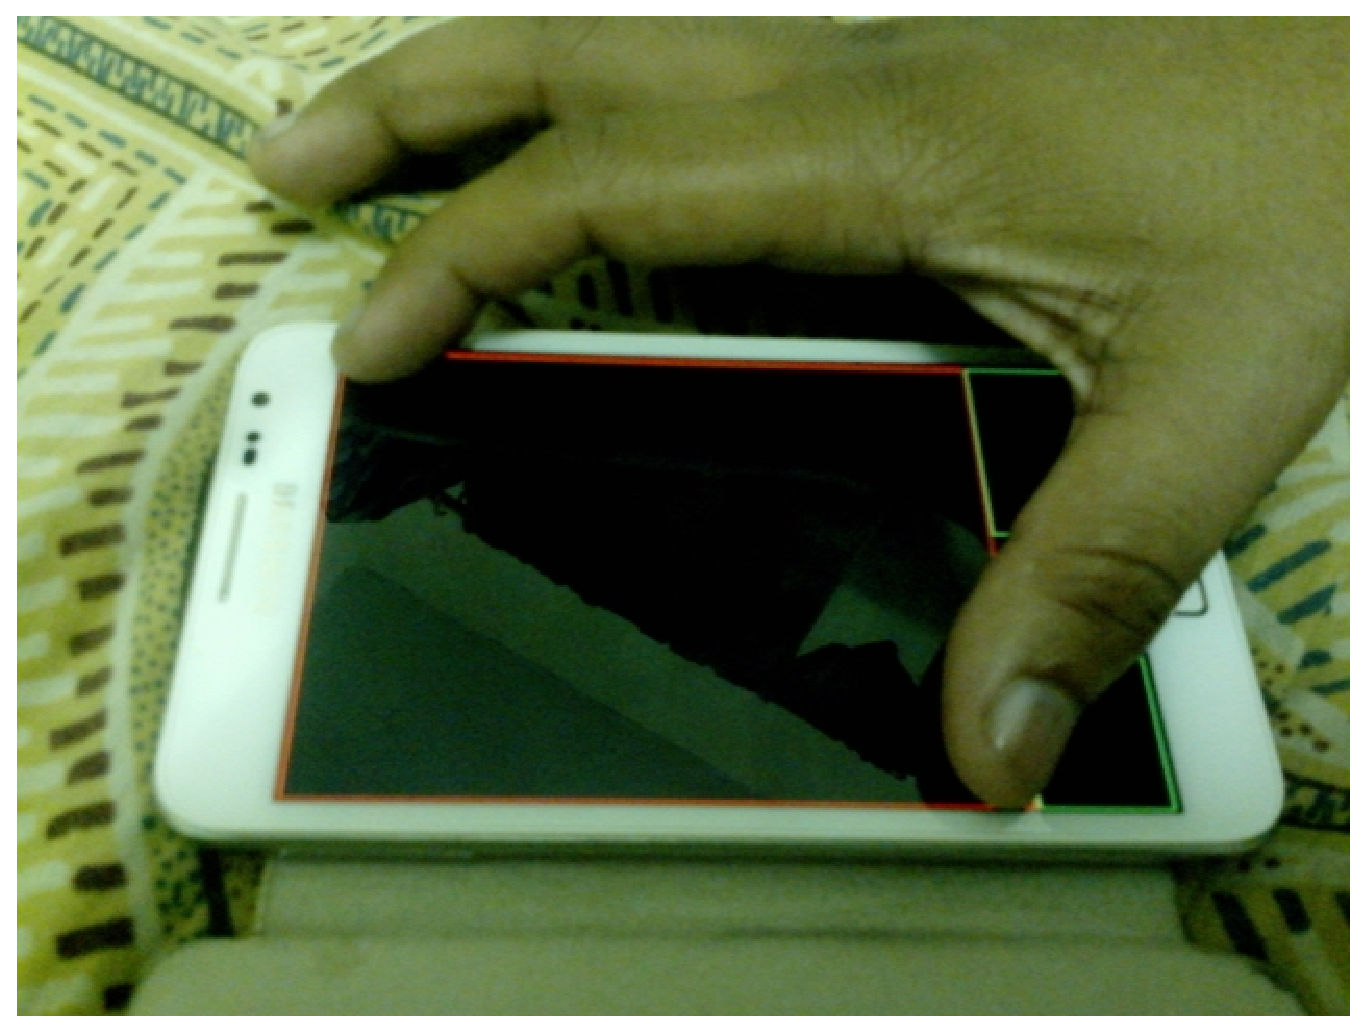
\includegraphics[width=120mm,height=45mm]{3.eps}
\caption{Two finger diagonal touch for locking the screen}
\end{figure*}
\begin{figure*}
\centering
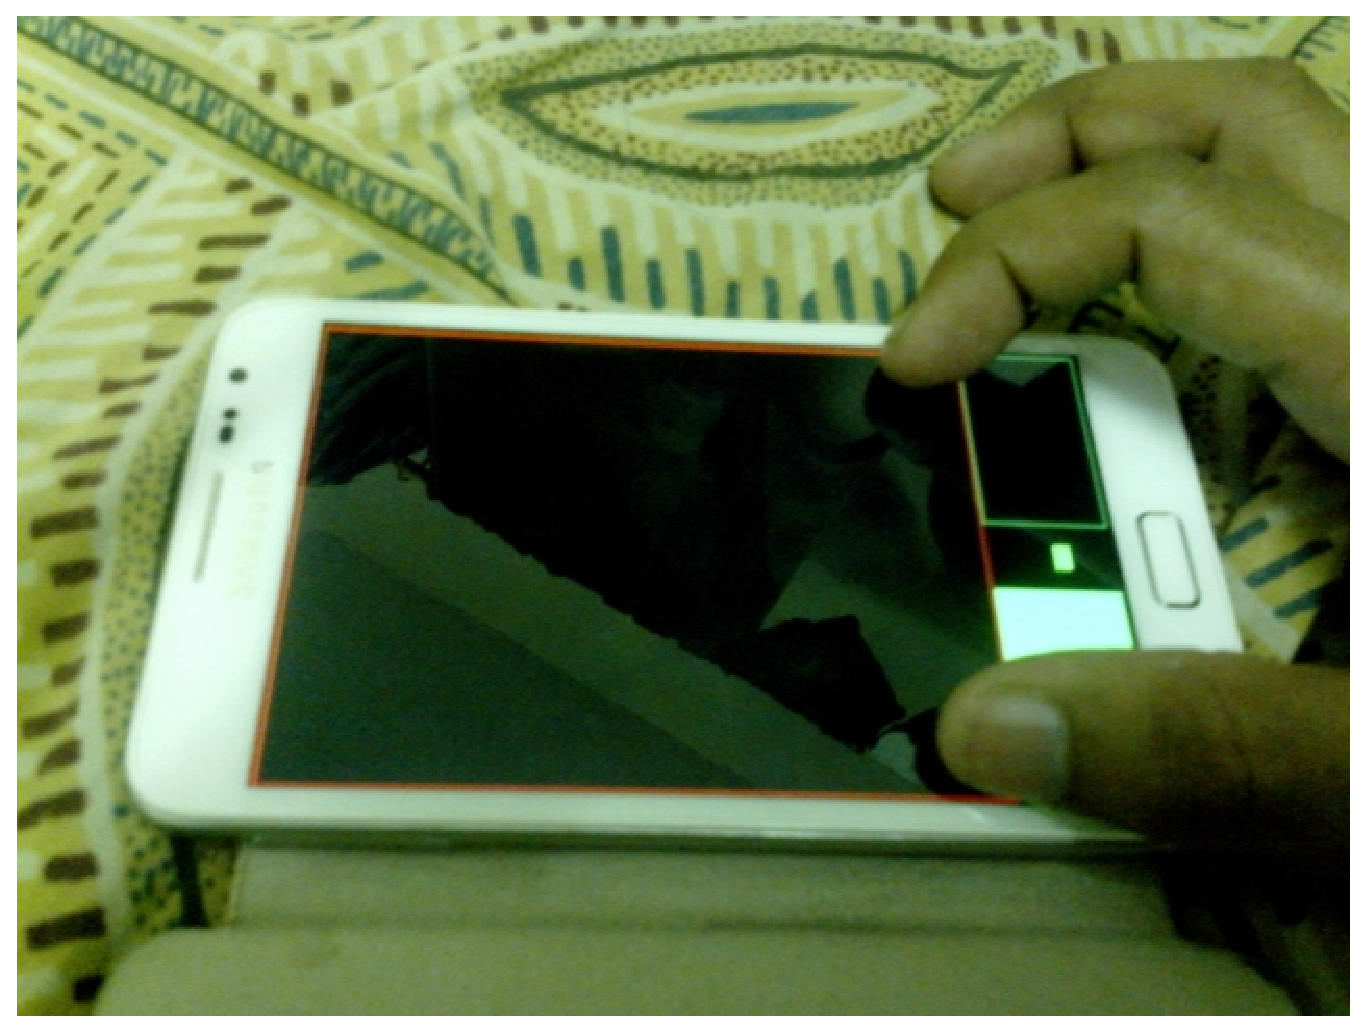
\includegraphics[width=120mm,height=45mm]{4.eps}
\caption{Two finger bottom touch for minimizing current window}
\end{figure*}
\begin{figure*}
\centering
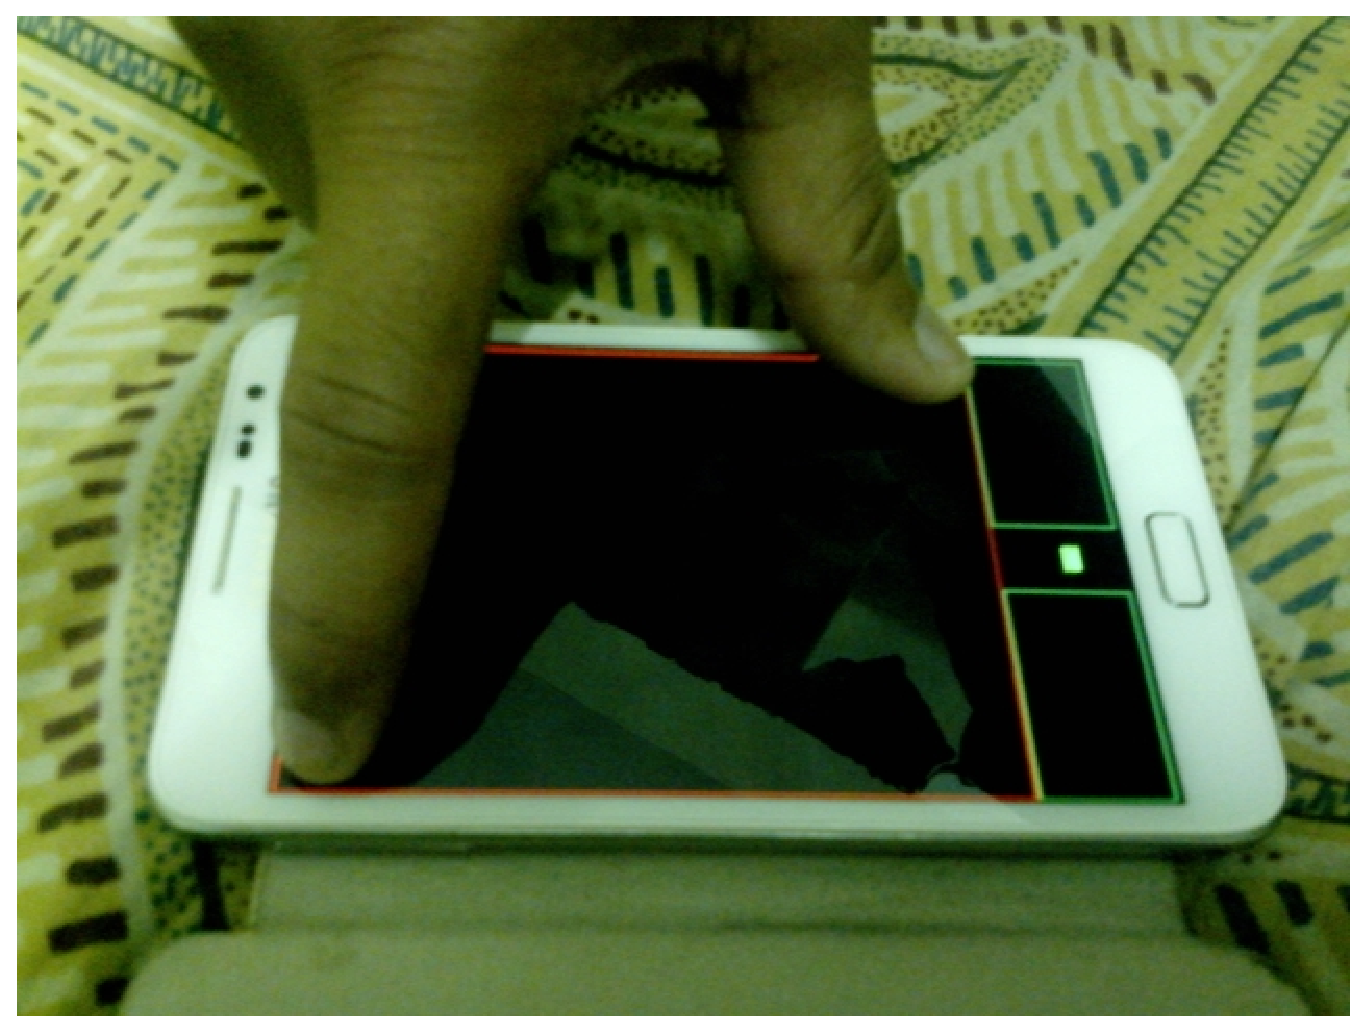
\includegraphics[width=120mm,height=45mm]{5.eps}
\caption{Two finger diagonal touch for opening task manager}
\end{figure*}
\begin{figure*}
\centering
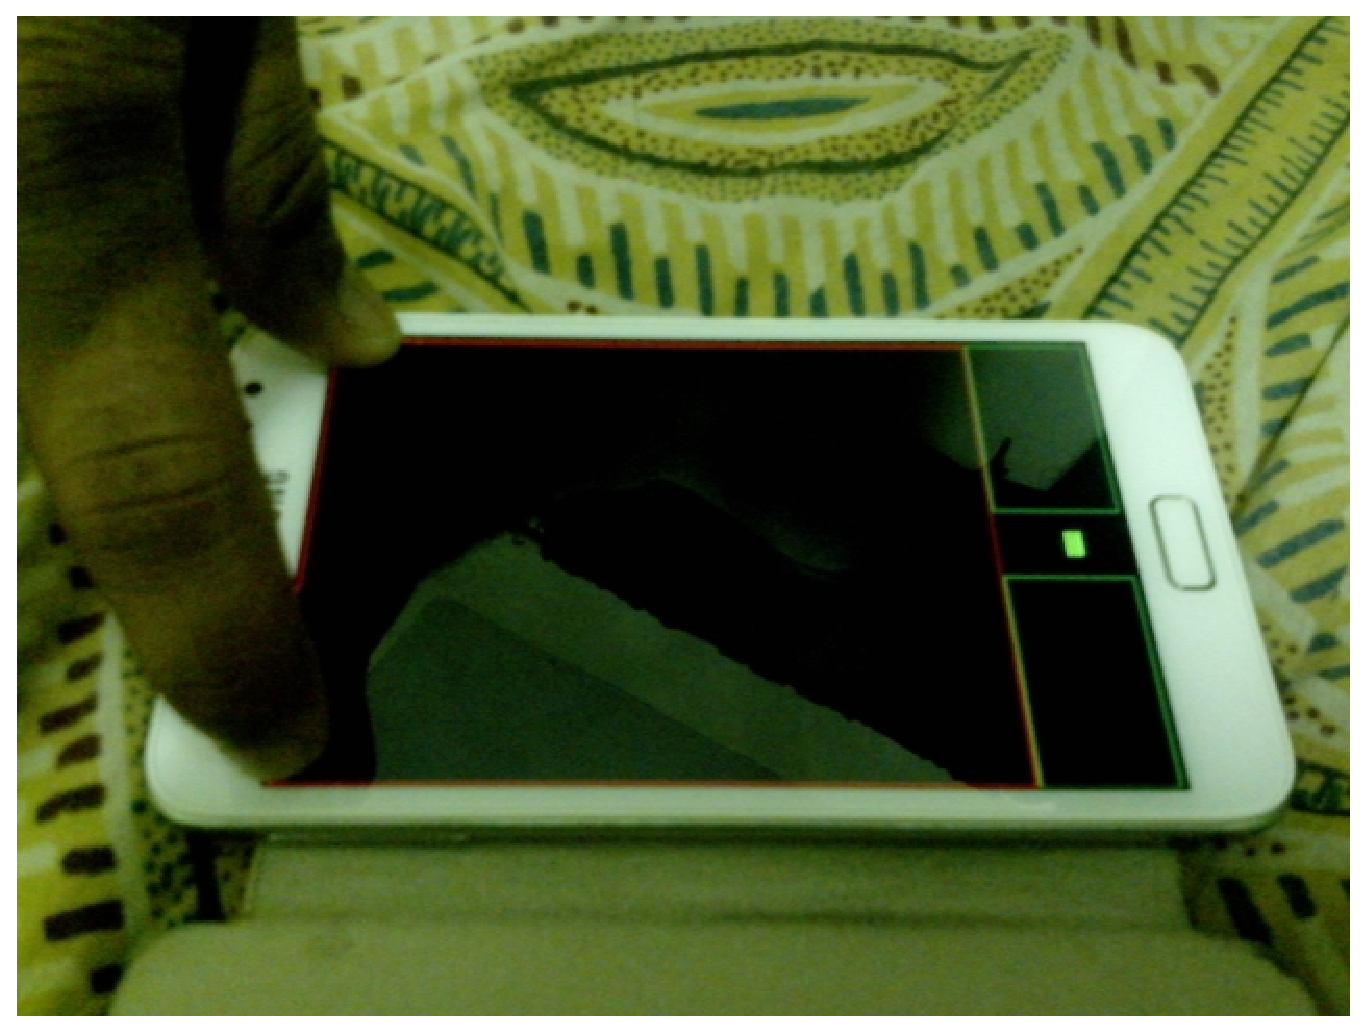
\includegraphics[width=120mm,height=45mm]{6.eps}
\caption{Two finger top touch for maximizing current window}
\end{figure*}
\begin{figure*}
\centering
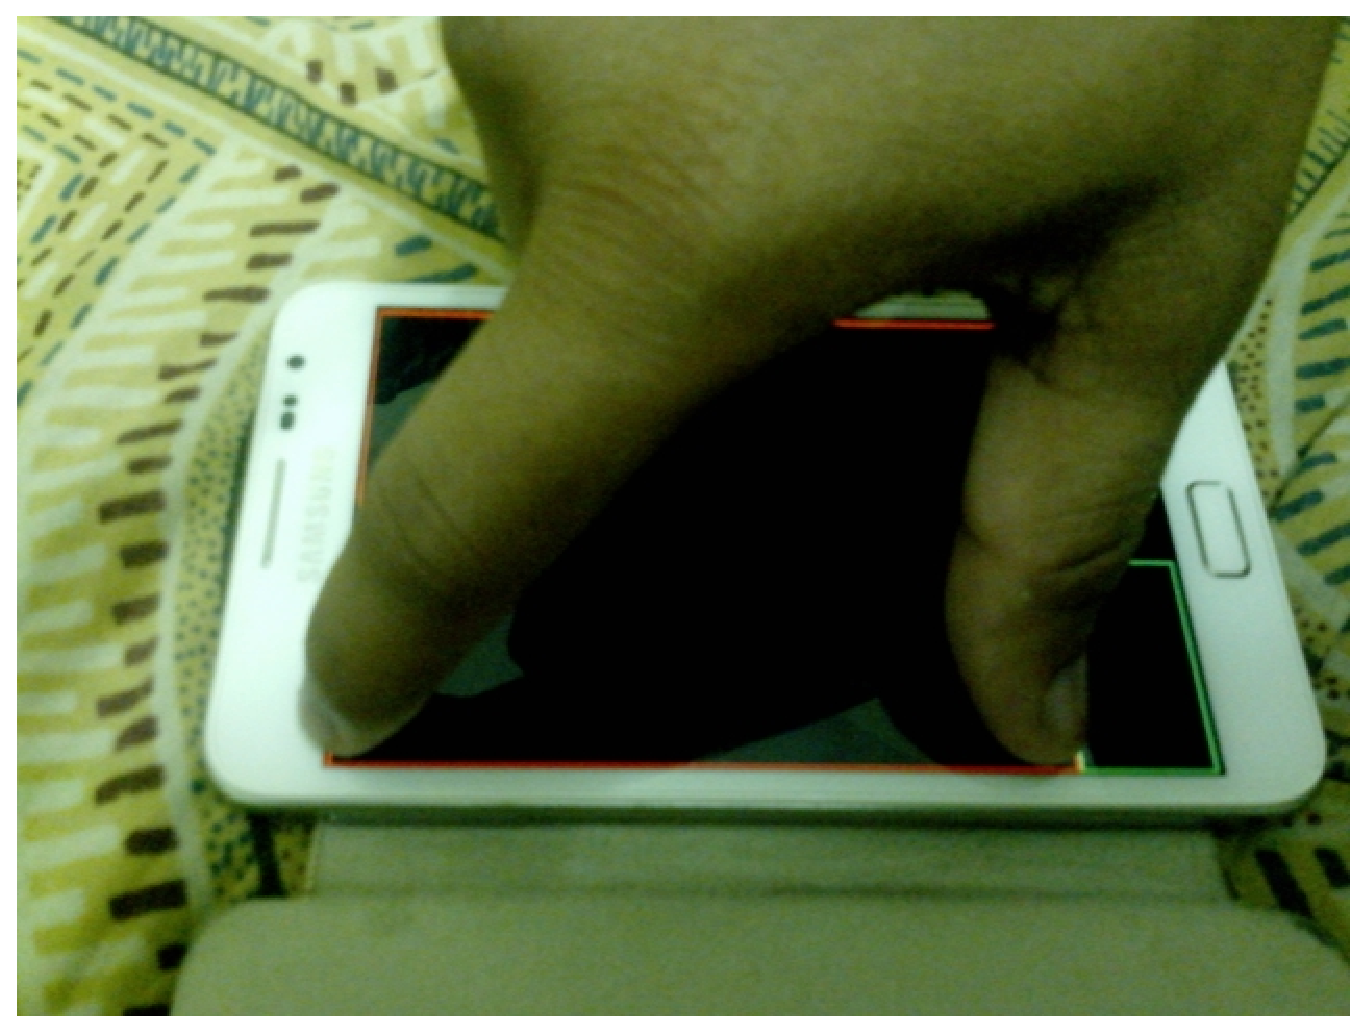
\includegraphics[width=120mm,height=45mm]{7.eps}
\caption{Two finger left touch for print command}
\end{figure*}
\begin{figure*}
\centering
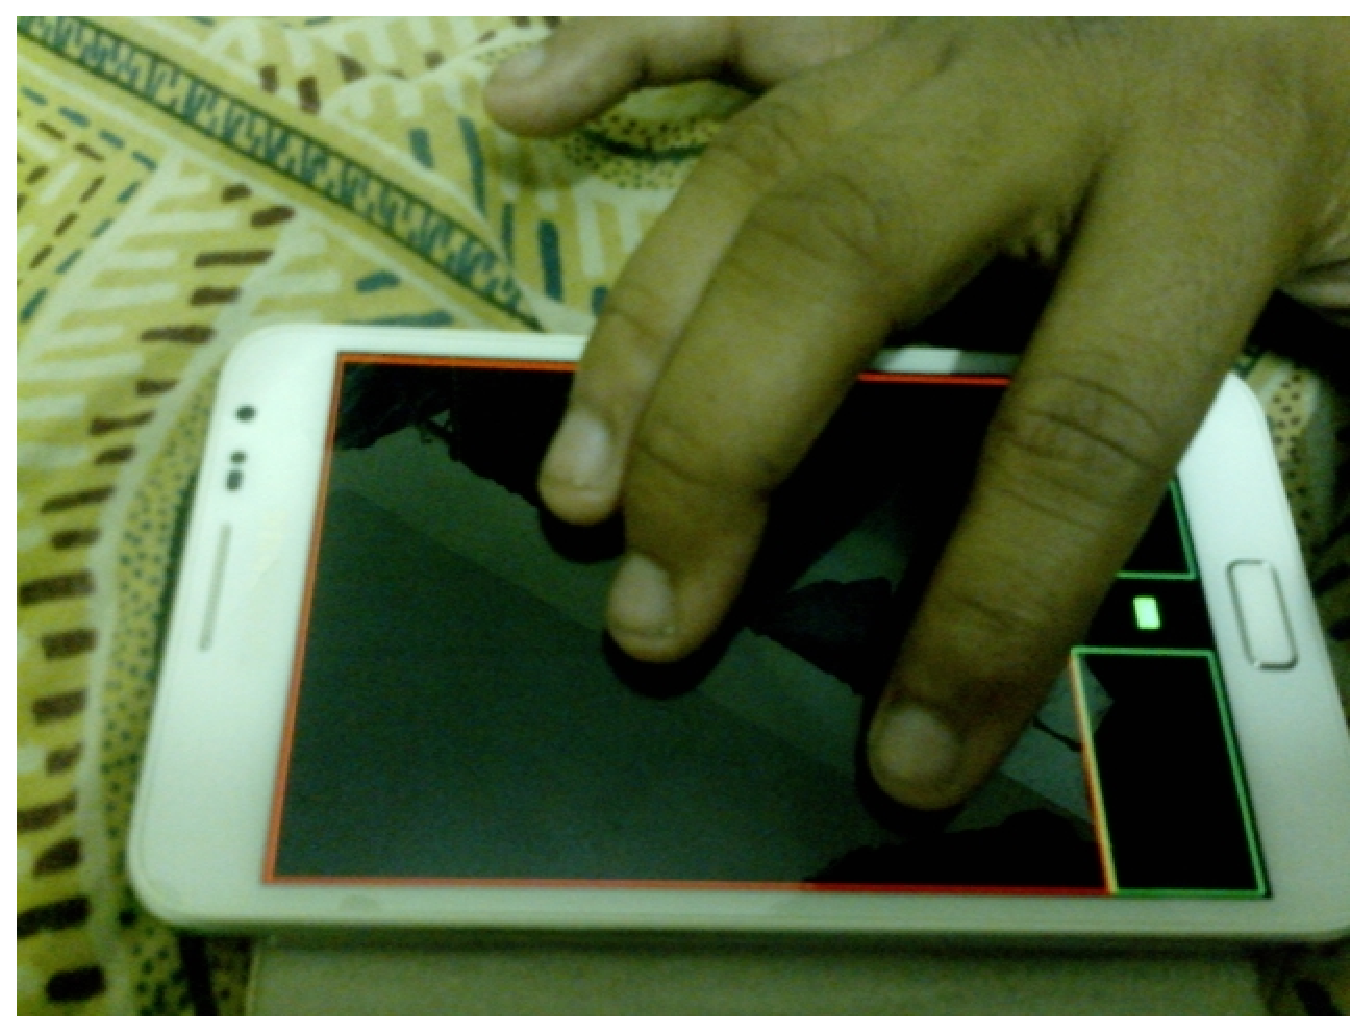
\includegraphics[width=120mm,height=45mm]{8.eps}
\caption{Three finger touch for switching between alternate windows}
\end{figure*}
\begin{figure*}
\centering
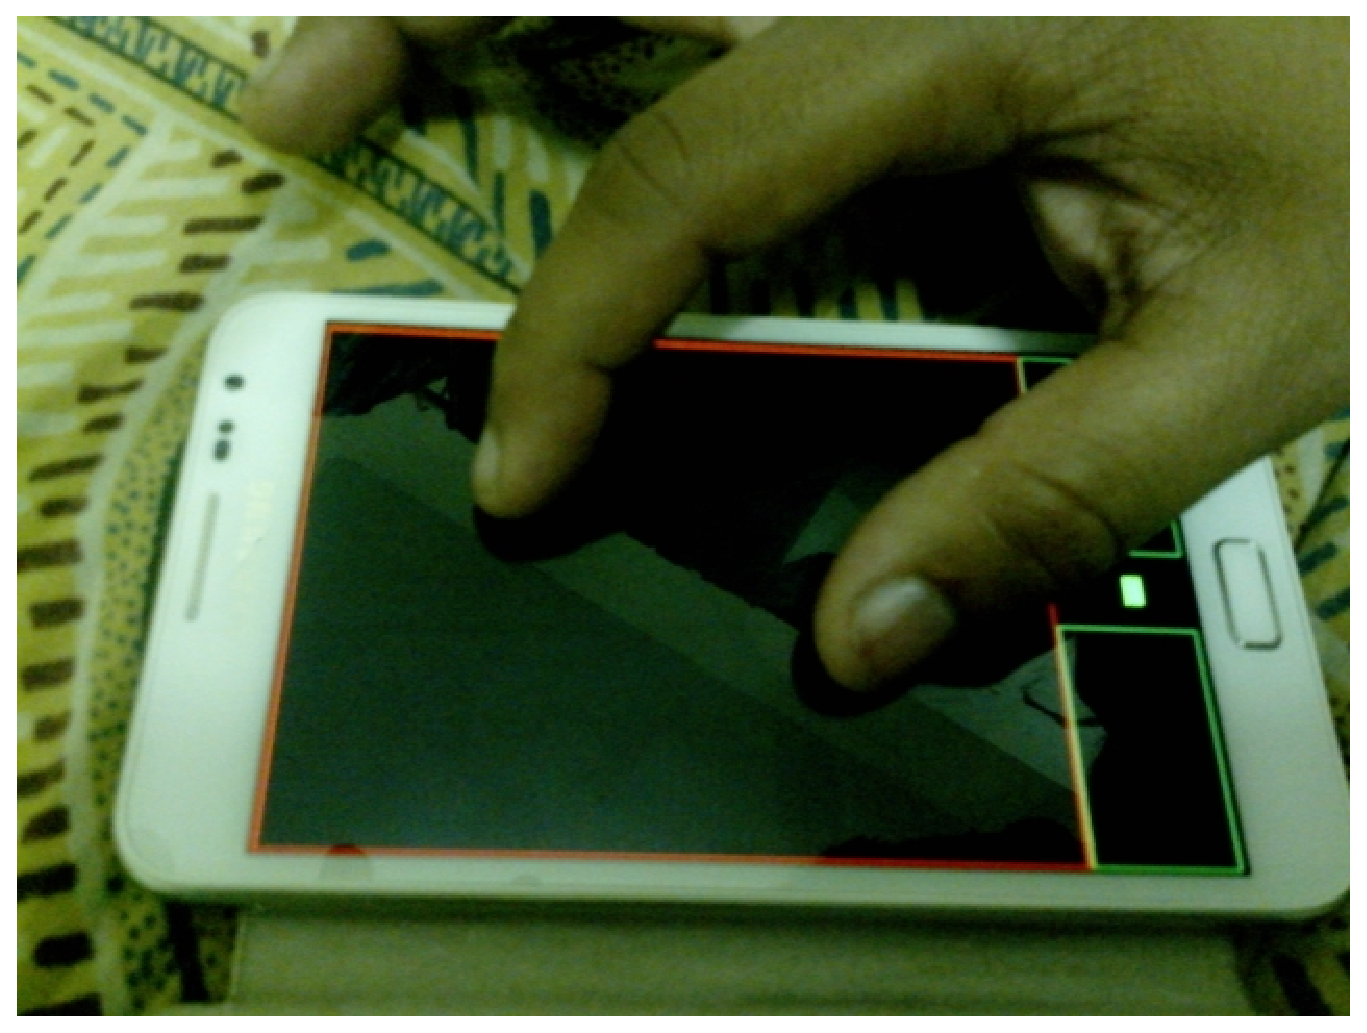
\includegraphics[width=120mm,height=45mm]{9.eps}
\caption{Two finger touch for pinch zooming}
\end{figure*}
\begin{figure*}
\centering
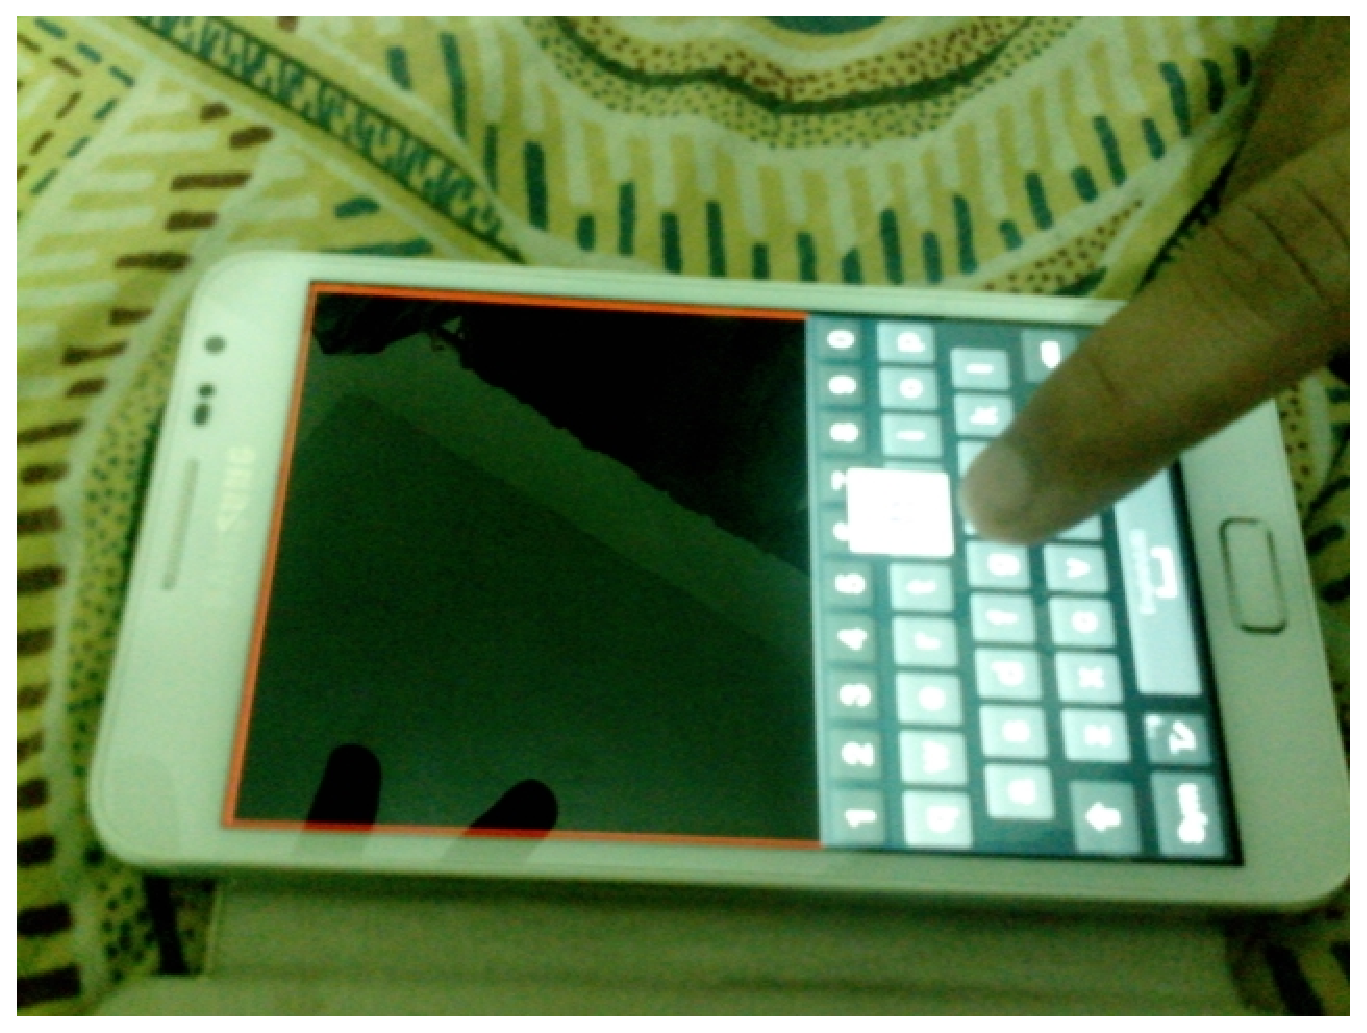
\includegraphics[width=120mm,height=45mm]{10.eps}
\caption{Keyboard Input}
\end{figure*}
\begin{figure*}
\centering
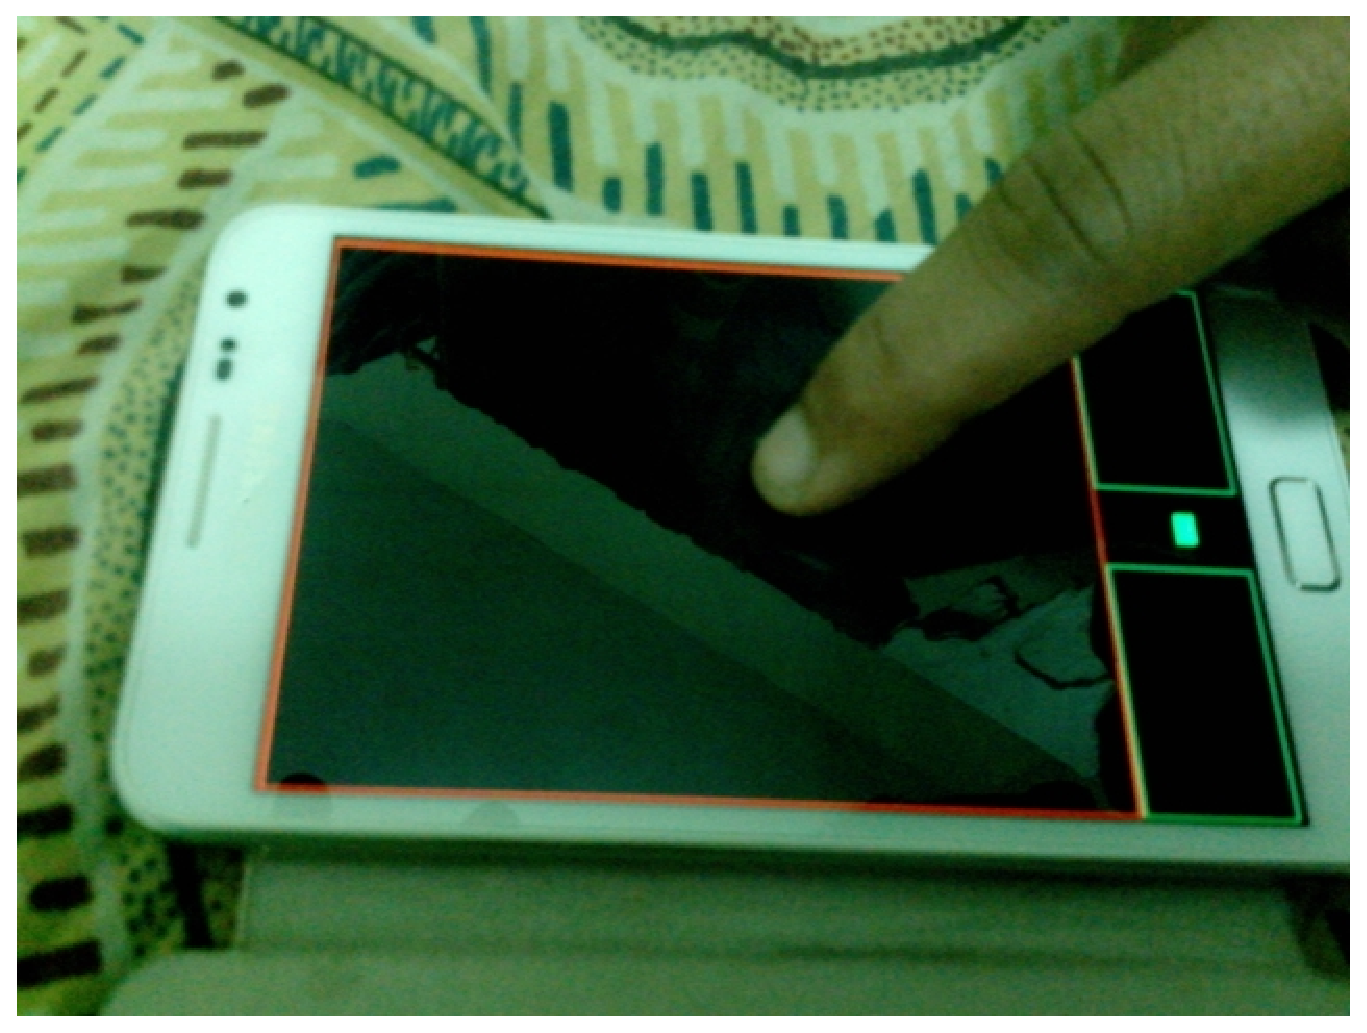
\includegraphics[width=120mm,height=45mm]{11.eps}
\caption{Single Touch Mouse Control}
\end{figure*}
\begin{figure*}
\centering
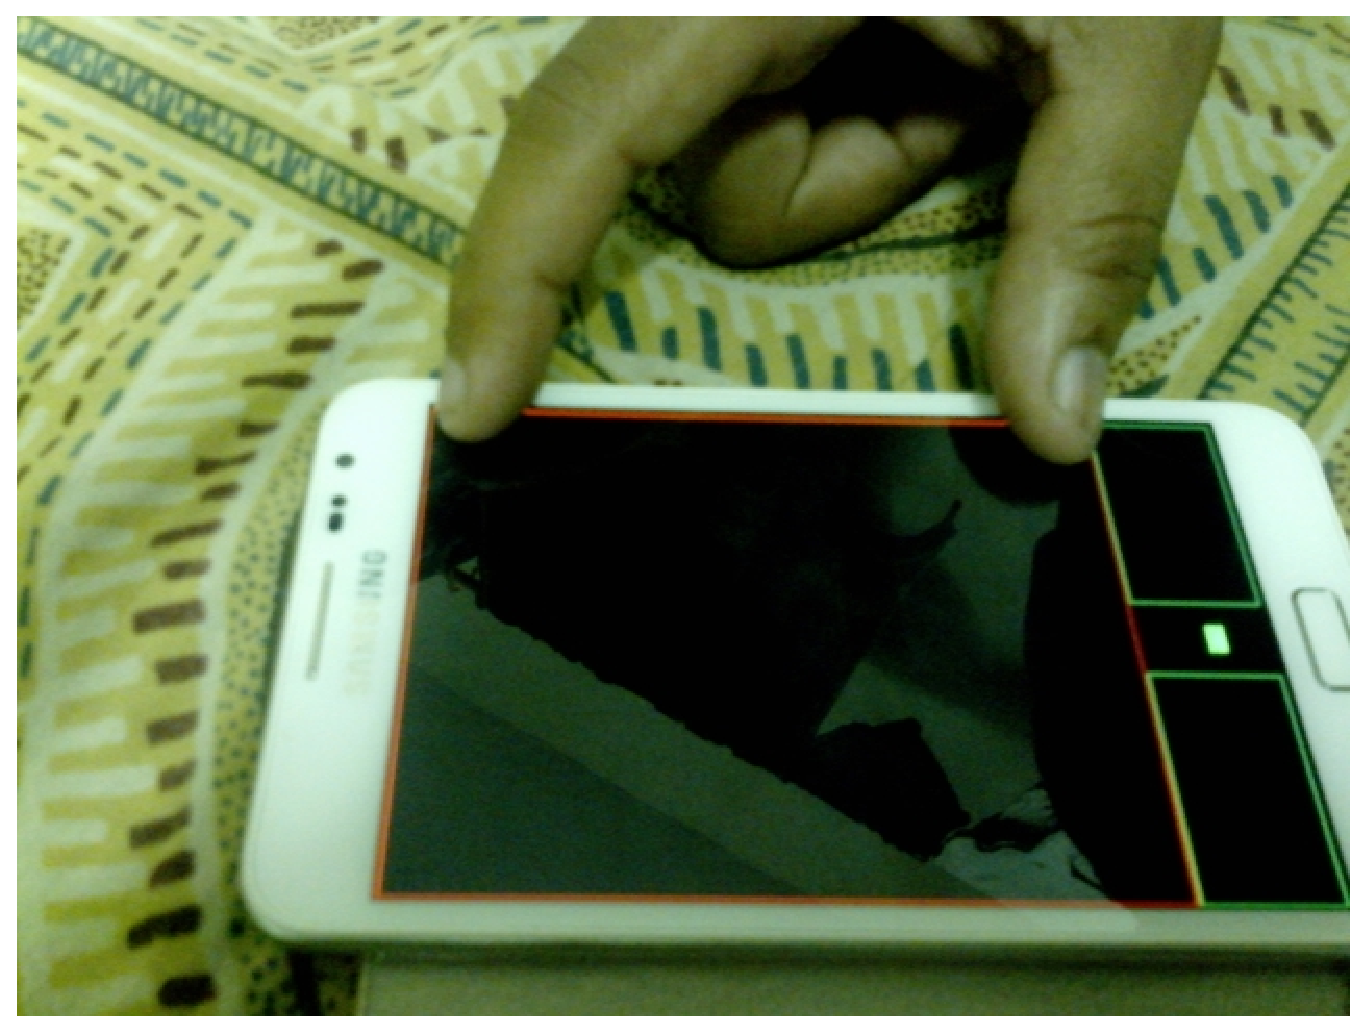
\includegraphics[width=120mm,height=45mm]{12.eps}
\caption{Two finger right touch for closing current window}
\end{figure*}
\begin{figure*}
\centering
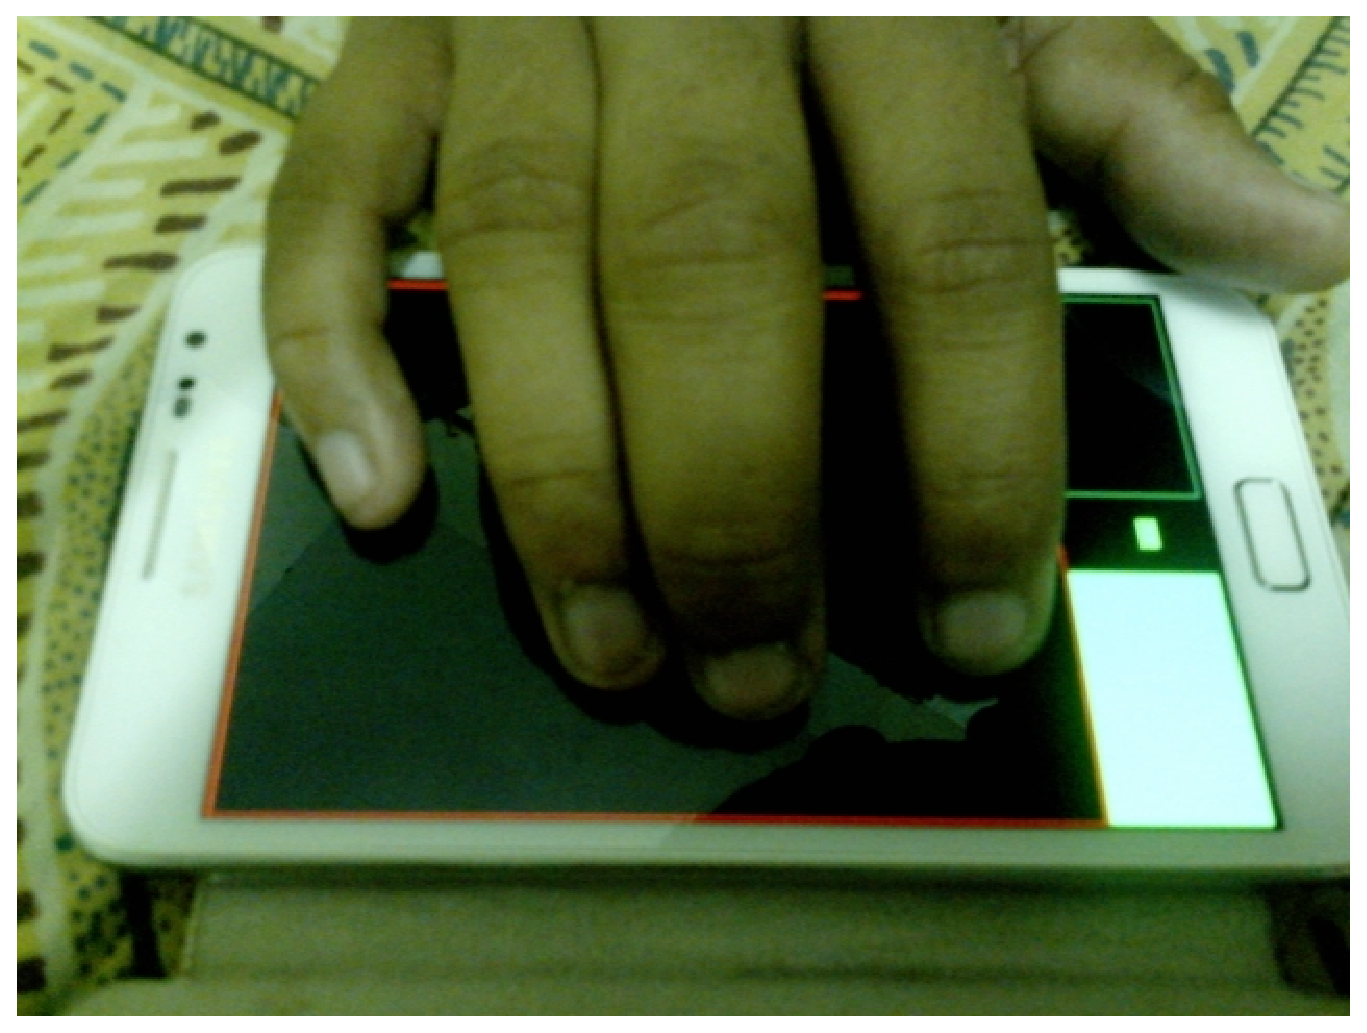
\includegraphics[width=120mm,height=45mm]{13.eps}
\caption{Four finger touch for capturing current screen display}
\end{figure*}
\begin{figure*}
\centering
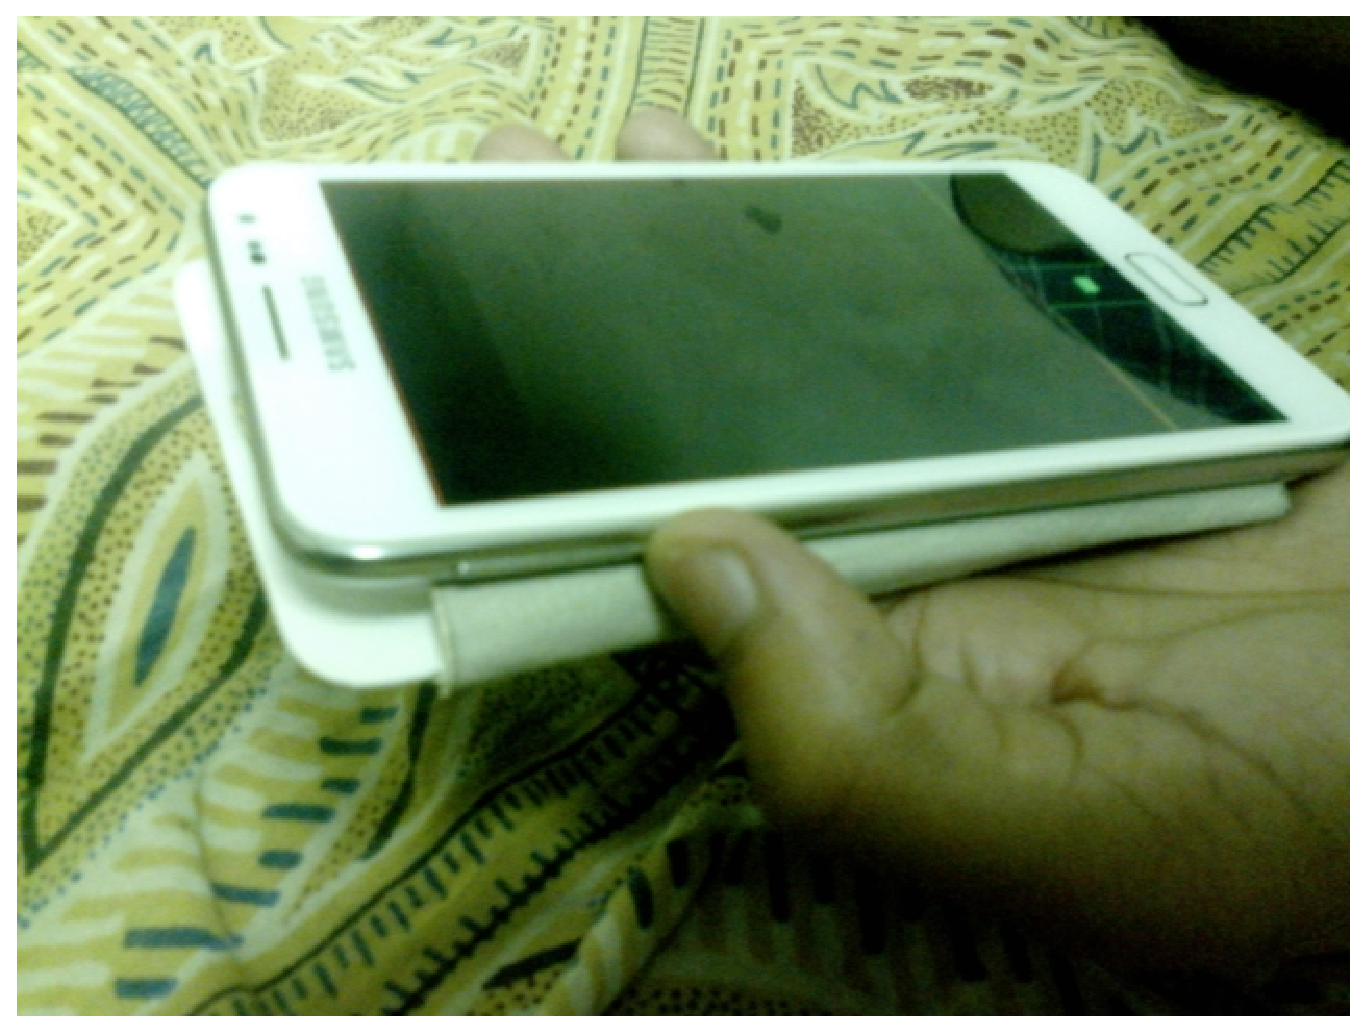
\includegraphics[width=120mm,height=45mm]{14.eps}
\caption{Volume Key Press Input}
\end{figure*}
\begin{figure*}
\centering
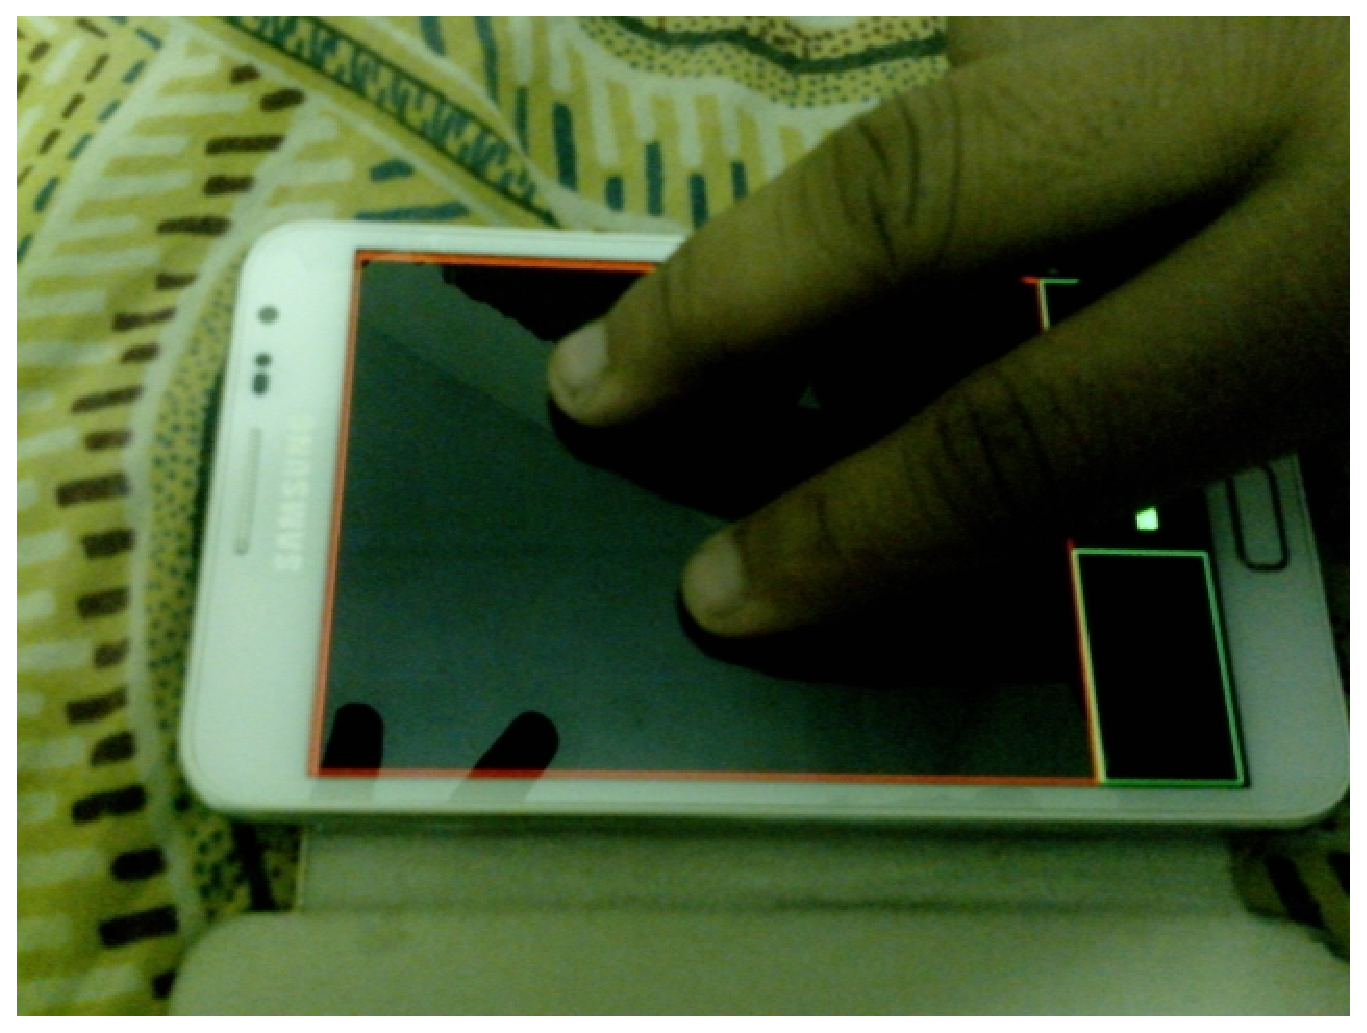
\includegraphics[width=120mm,height=45mm]{15.eps}
\caption{Double Finger Scroll}
\end{figure*}

\section{Implementation Details}
The Android device is our client and the script running on the laptop is our server.\\
Server side implementation is done in Java and Client side implementation is done using Android APIs.\\
We now discuss some of the important elements of MyGesture.
\subsection{OSC Message}
Open Sound Control(OSC) is a content format for messaging among computers, sound synthesizers, and other multimedia devices that are optimized for modern networking technology. OSC messages are commonly transported across the internet and within home and studio subnets using (UDP/IP, Ethernet).\\\\
The unit of transmission of OSC is an OSC Packet. Any application that sends OSC Packets is an OSC Client; any application that receives OSC Packets is an OSC Server.\\
An OSC packet consists of its contents, a contiguous block of binary data, and its size, the number of 8-bit bytes that comprise the contents. The size of an OSC packet is always a multiple of 4.\\
The underlying network that delivers an OSC packet is responsible for delivering both the contents and the size to the OSC application. \\
An OSC packet can be naturally represented by a datagram by a network protocol such as UDP. In a stream-based protocol such as TCP, the stream should begin with an int32 giving the size of the first packet, followed by the contents of the first packet, followed by the size of the second packet, etc.\\\\
An OSC message consists of an OSC Address Pattern followed by an OSC Type Tag String followed by zero or more OSC Arguments. An OSC Address Pattern is an OSC-string beginning with the character '/' (forward slash).

\subsection{WiFi}
We have used WiFi instead of bluetooth because of its longer range connectivity and higher access speed. This would help us to extend the app for high data streaming without much changes. Also the WiFi is more secure as compared to Bluetooth.

\subsection{Android Classes}
We have mainly used following two classes for giving touch gestures.
\begin{itemize}
\item \textbf{MotionEvent:} Object used to report movement(mouse, pen, finger, trackball) events. Motion events may hold either absolute or relative movements and other data, depending on the type of device. 
\item \textbf{Sensor:} Most Android-powered devices have built-in sensors that measure motion, orientation, and various environmental conditions.
\end{itemize}
The description of the above two functionalities and few others is summarized through the table below:
\begin{table}[!h]
\centering

    \caption{Android Classes at a glance}     % NOTE!  caption goes _before_ the table contents !!
    \label{tab:font-sizes}

    \begin{small}
    \begin{tabular}{|l|l|}
    \hline
    \cline{2-2}
    {\bfseries  Class/Function}         & {\bfseries Description}             \\
	\hline
    TYPE\_ACCELEROMETER	&	Measures the acceleration     \\
    &  force in m/s2;applied to all \\
    & three physical axes, including  \\
    & the force of gravity \\
    \hline
    TYPE\_PRESSURE	&	Measures the ambient 	     \\
    & air pressure in hPa or mbar  \\   
    \hline
    ACTION\_DOWN	&	 Pressed gesture has \\
    & started;motion contains \\
    & initial starting location \\
    \hline
    ACTION\_MOVE	&	 A change has happened  \\
    & during a press gesture \\
    \hline
    ACTION\_UP	&	 Pressed gesture has  \\
    & finished;motion contains  \\
    & final release location \&  \\
	& intermediate points \\
    \hline
    ACTION\_MASK	&	 Bit mask of the parts of  \\
    & the action code that are \\
    & the action itself \&  \\
    \hline
    ACTION\_CANCEL	&	The current gesture   \\
    & has been aborted \\
    \hline
    ACTION\_OUTSIDE	&	A movement has happened    \\
    & outside of the normal  \\
    & bounds of the UI element \\
    \hline
    ACTION\_POINTER\_UP	&	A non-primary   \\
    & pointer has gone up  \\
    \hline
    connect()	&	Starts a peer-to-peer    \\
    & connection with a device  \\
    & with the specified configuration \\
    \hline
    discoverPeers()	&	Initiates peer discovery     \\
    \hline
    requestPeers()	&	Requests the current list   \\
    & of discovered peers \\
    \hline
    \end{tabular}
    \end{small} 
\end{table}

\subsection{Integral Steps}
The first step is to discover the available servers which is done by opening a new multicast socket at port number 57111. The client then  sends a packet for \emph{id\_request}. This discovers all the available hosts and then we display them on the android screen.\\
Next, we select one of the available servers, after which a datagram socket is opened on the client for sending the messages. The socket is opened on the port 57111.\\
On clicking connect button, it checks whether the entered IP address is valid or not and then it sets the IP in Settings.class and then opens the \emph{PadActivity}.\\
This is the main screen on the client side through which all the touch gestures and keyboard activities are given as input. All the event listeners such as Accelerometer, MotionListener and KeypressListener are active when we enter PadActivity mode.\\
WrappedMotionEvent extends the MotionActivity class for providing multi-touch functionalities like getting pointer count of all the touches and the $x$ and $y$ coordinates of each pointer.

\subsection{Server Script}
The Java script on the server side mainly uses a class called \emph{Robot} for performing all the different activities assigned for touch gestures.\\
This class is used to generate native system input events for the purposes of test automation, self-running demos, and other applications where control of the mouse and keyboard is needed. The primary purpose of Robot is to facilitate automated testing of Java platform implementations.\\
The server side also has a port which keeps on listening for any OSC packet. This information is then filtered and then passed to the desired Robot event module.

\subsection{Hardware}
Our framework was tested on the following devices(a smart phone running Android 4.1.2, and a laptop running Windows 7).
\begin{itemize}
\item \textbf{Smartphone: Samsung Galaxy Note N7000} with Dual-core 1.4 GHz ARM Cortex-A9 Processor with 1GB RAM, running Android JellyBean 4.1.2
\item \textbf{Laptop: HP} with Intel Core i5 Processor, 4GB RAM, running Windows 7\\
\end{itemize}

\subsection{Running MyGesture}
The server side script is a runnable \emph{jar} file.\\
The client side script is an Android code which can be packed inside a \emph{apk} file and can be directly installed on an Android device.\\
Once the application is opened on the android device, the server needs to be started on the laptop. We also need to ensure that system firewall allows packet transfer through this application. The laptop and mobile, both should have WiFi device in ON mode.\\

\section{Conclusion}
Mouse Sensitivity was one of the main problem faced during this work, because we needed to map a higher resolution screen to a lower resolution space on the Android screen. Since we have many two finger gestures, differentiating between them was a major challenge. Hence, dividing the screen for each input gesture was also taken into consideration so that gestures donot overlap.\\
Drawing gestures also posed a challenge because in case of a gesture which was some figure, it became ambiguous for us to decipher whether the user intended to move the mouse in that way or he wanted the assigned action for that gesture to invoke.\\

\section{Future Work}
As a continuation of this work, we would like to integrate with our android application, input patterns and codes, which correspond to specific actions on a laptop. E.g. writing "M" on touchpad and correspondingly opening media player in laptop.\\ We would also like to add music streaming to and fro between android device and laptop. We will also put efforts for displaying the screen of the target PC on the android phone itself for the purpose of better visualisation.\\
We can also integrate bluetooth connectivity into our system providing us more options for connectivity and opening a path for connection of two android devices.\\

\section{Acknowledgement}
We would like to show our sincere gratitude towards Prof. R.K. Ghosh, Professor, Computer Science and Engineering
Department, IIT Kanpur for his motivation to do this work and becoming our advisor for this work. We would also like to thanks Dr. Maitreya Natu, Scientist, Tata Research Design and Development Center(TRDDC), Pune, India for his valuable inputs. We would
also like to thank our all friends and TAs who have helped us directly or indirectly throughout this project. We would also like to thank CSE Department, IIT Kanpur for providing such courses as CS634 where we get involved in projects such as this which enables us to lean mobile networking and related applications.


\bibliographystyle{IEEEtr}

\bibliography{report} 
\nocite{*}
\end{document}
